%% -*- TeX-master: t -*-

% \documentclass{acm_proc_article-sp}
\documentclass{sig-alternate}

% remove this before creating camera-ready final copy!
\setlength{\overfullrule}{5pt}

\newcommand{\thetitle}[0]{Statistical Debugging Using Compound Boolean Predicates}
\newcommand{\wraptitle}[0]{Statistical Debugging Using \\ Compound Boolean Predicates}

\pagenumbering{arabic}

%%%%%%%%%%%%%%%%%%%%%%%%%%%%%%%%%%%%%%%%%%%%%%%%%%%%%%%%%%%%%%%%%%%%%%%%
%%
%% standard texmf packages
%%

% font selection
\usepackage[T1]{fontenc}
\usepackage{courier}
\usepackage[scaled]{helvet}
\usepackage{mathptmx}

\usepackage{booktabs}
\usepackage{flushend}
\usepackage{graphicx}
\usepackage{hyphenat}
\usepackage{nicefrac}
\usepackage{paralist}
\usepackage{subfig}
\usepackage[dvips]{thumbpdf}
\usepackage{xspace}

\usepackage[
bookmarks,
breaklinks,
letterpaper,
pdftitle={\thetitle},
pdfauthor={Piramanayagam Arumuga Nainar, Ting Chen, Jake Rosin, and Ben Liblit},
% pdfsubject={D.2.4 [Software Engineering]: Software/Program Verification -- statistical methods; D.2.5 [Software Engineering]: Testing and Debugging -- debugging aids, distributed debugging, monitors, tracing; I.5.2 [Pattern Recognition]: Design Methodology -- feature evaluation and selection},
% pdfkeywords={bug isolation, random sampling, invariants, feature selection, statistical debugging},
]{hyperref}

\captionsetup[table]{position=top}


%%%%%%%%%%%%%%%%%%%%%%%%%%%%%%%%%%%%%%%%%%%%%%%%%%%%%%%%%%%%%%%%%%%%%%%%
%%
%% unique to this report
%%

\newcommand{\figurename}[0]{Figure}
\newcommand{\tablename}[0]{Table}

\newdef{defn}{Definition}
\newcommand{\defnautorefname}[0]{Definition}

\newcommand{\Importance}[0]{\mathit{Importance}\xspace}
\newcommand{\Increase}[0]{\mathit{Increase}\xspace}
\newcommand{\NumF}[0]{\mathit{NumF}\xspace}
\newcommand{\effort}[0]{\mathit{effort}\xspace}

\newcommand{\obs}[2]{#1(\text{$#2$ obs})}
\newcommand{\obsFalse}[2]{#1(\text{$\bar{#2}$})}

\newcommand{\true}[0]{\mathit{true}\xspace}
\newcommand{\false}[0]{\mathit{false}\xspace}
\newcommand{\unknown}[0]{\mathit{unknown}\xspace}

\newcommand{\ub}[1]{\uparrow#1}
\newcommand{\lb}[1]{\downarrow#1}

\newcommand{\prog}[1]{\texttt{#1}}
\newcommand{\func}[1]{\texttt{#1}}

\renewcommand{\sectionautorefname}[0]{Section}
\renewcommand{\subsectionautorefname}[0]{\sectionautorefname}
\renewcommand{\subsubsectionautorefname}[0]{\sectionautorefname}
\newcommand{\subtableautorefname}[0]{\tableautorefname}

\newcommand{\Max}[2]{\textbf{max(}#1, #2\textbf{)}}
\newcommand{\Min}[2]{\textbf{min(}#1, #2\textbf{)}}

%%%%%%%%%%%%%%%%%%%%%%%%%%%%%%%%%%%%%%%%%%%%%%%%%%%%%%%%%%%%%%%%%%%%%%%%
%%
%% front matter
%%

\title{%
  \wraptitle%
  \thanks{This research was supported in part by AFOSR Grant
    FA9550-07-1-0210 and NSF Grant CCF-0621487.}}

\newcommand{\mailto}[1]{\href{mailto:#1@cs.wisc.edu}{#1}}

\numberofauthors{1}
\author{\alignauthor
  Piramanayagam Arumuga Nainar \qquad Ting Chen \qquad Jake Rosin \qquad Ben Liblit \\
  \affaddr{Computer Sciences Department} \\
  \affaddr{University of Wisconsin--Madison} \\
  \email{\{\mailto{arumuga},\mailto{tchen},\mailto{rosin},\mailto{liblit}\}@cs.wisc.edu}}

%%%%%%%%%%%%%%%%%%%%%%%%%%%%%%%%%%%%%%%%%%%%%%%%%%%%%%%%%%%%%%%%%%%%%%%%
%%
%%  document body
%%

\begin{document}

\conferenceinfo{ISSTA'07,} {July 9--12, 2007, London, England, United Kingdom.}
\CopyrightYear{2007}
\crdata{978-1-59593-734-6/07/0007} 

\maketitle

\begin{abstract}
Cooperative Bug Isolation (CBI) is a technique to find bugs in programs that analyzes data collected from program executions.  At each program point, CBI identifies boolean expressions, called as predicates, to be instrumented.  We augment CBI's bug predictive ability by combining these predicates using logical operators (conjunction and disjunction).  The motivation is that a complex predicate will provide more information to the programmer by narrowing down possible program states.  Our experimental results show that the scores of complex predicates are usually higher or atleast comparable to single predicates.  This makes them good indicators of bugs.  We discuss a new metric that uses program structure to quantify the usefulness of complex predicates.  Using this metric, we could eliminate a large number of spurious predicates from consideration.  Finally we discuss the effect of sparse random sampling on the usefulness of complex predicates.

\end{abstract}

\category{D.2.4}{Software Engineering}{Software/Program Verification}[statistical methods]
\category{D.2.5}{Software Engineering}{Testing and Debugging}[debugging aids, distributed debugging, monitors, tracing]
\category{I.5.2}{Pattern Recognition}{Design Methodology}[feature evaluation and selection]

\terms{Experimentation, Reliability}

\keywords{statistical bug isolation,
          three-valued logic,
          debugging effort metrics,
          dynamic feedback analysis
          }

\input{introduction}
% -*- TeX-master: "master" -*-

\section{Background}
\label{sec-background}
CBI uses lightweight instrumentation to collect feedback reports that contain truth values of predicates in an execution as well as the outcome (e.g., crash or non-crash) of the execution.  Large numbers of reports are collected, then analyzed using statistical debugging techniques.  These techniques identify \emph{bug predictors}: predicates that, when true, herald failure due to a specific bug.  Bug predictors highlight areas of the code that are related to program failure and so provide information that is useful when correcting program faults.  Feedback reports can be collected from deployed software in the hands of end users, who may encounter bugs not identified in program testing.  CBI can therefore be used to monitor software after its release and help direct program patches by identifying bugs as they manifest in the field.

\subsection{Finding Bug Predictors}
\label{sec-elimalg}
The feedback report for a particular program execution is formed as a bit-vector, with two bits for each predicate (\emph{observed} and \emph{true}), and one final bit representing success or failure.  If generated in experimental or testing conditions these feedback reports are likely to be complete; when instrumented code is distributed to end users predicates are usually sampled infrequently to reduce computational overhead.  Previous experiments \cite{Liblit:2003:BIRPS} have determined that sampling rates of \nicefrac{1}{100} to \nicefrac{1}{1,000} are most realistic for deployed use.

Using these reports, CBI assigns a score to all available predicates and identifies the single best predictor among them (see \autoref{sec-scoring}).  It is assumed that this predictor corresponds to one important bug, though other bugs may remain.    This top predictor is recorded, and then all feedback reports where it was true are removed from consideration under the assumption that fixing the corresponding bug will change the behavior of runs in which the predictor originally appeared.  The next best predictor among the remaining reports is then identified, recorded, and removed in the same manner.  This iterative process terminates either when no undiagnosed failed runs remain, or when no more failure-predictive predicates can be found.

This process of iterative elimination maps each predictor to a set of program runs.  Ideally each such set corresponds to the expression of a distinct bug; unfortunately this is not always the case.  Due to the statistical nature of the analysis, along with incomplete feedback reports resulting from sparse sampling rates, a single bug could be predicted by several top-ranked predicates, and predictors for less prevalent bugs may not be found at all.

The output of the analysis is a list of predicates that had the highest score during each iteration of the elimination algorithm, as well as a complete list of predicates and their scores before any elimination is performed.  These lists may be used by a programmer to identify areas of the program related to faulty behavior.  Liblit et al.\ employed this method to discover previously unknown bugs in several widely-used applications \cite{Liblit:2003:BIRPS,Liblit:2005:SSBI}.

CBI output can also be used as input to an automated analysis tool, such as \textsc{BTrace} \cite{Lal:2006:POPAD}. \textsc{BTrace} finds the shortest control- and dataflow-feasible path in the program that visits a given set of bug predictors.  This analysis allows a programmer to examine the fault-predicting behavior even if the connection to a bug is not easily identifiable, or if the predictors are numerous or complex enough to overwhelm a programmer examining them directly.

\subsection{Scoring Predicates}
\label{sec-scoring}
This section provides a brief overview of the numeric scores used to identify the best predictor from a set of predicates.  For a detailed discussion on this topic, the reader should refer to Liblit et al.\ \cite{Liblit:2005:SSBI}.  A good predictor should be both \emph{sensitive} (accounts for many failed runs) and \emph{specific} (does not mis-predict failure in successful runs).  Assigning scores based on sensitivity will result in \emph{super-bug predictors}, which include failures from more than one bug.  Super-bug predictors are highly non-deterministic, since they are not specific to any single cause of failure, and rarely provide useful debugging information.  Scoring predicates based on specificity instead results in \emph{sub-bug predictors}.  A sub-bug predictor accounts for a portion of the failures caused by a bug, but not all.  Unlike super-bug predictors, sub-bug predictors that account for a significant sub-set of failures can be useful in debugging, although perfect predictors are of course preferred.  Sensitivity and specificity are balanced using a numeric $\Importance$ score computed as follows.

The truth values of a predicate $p$ from all the runs can be aggregated into four values:

\begin{enumerate}
\item $\obs{S}{p}$ and $\obs{F}{p}$, respectively the number of successful and failed runs in which the value of $p$ was evaluated.
\item $S(p)$ and $F(p)$, respectively the number of successful and failed runs in which the value of $p$ was evaluated and was found to be true.
\end{enumerate}

Using these values, two scores of bug relevance are calculated:
\begin{description}
\item[Sensitivity:] $\log{(F(p))} / \log{(\NumF)}$ where $\NumF$ is the total number of failing runs.  A good predictor must predict a large number of failing runs.
\item[Specificity:] $\Increase(p)$.  The amount by which $p$ being true increases the probability of failure over simply reaching the line where $p$ is defined.  It is computed as follows:

  \begin{equation*}
    \label{eqn1}
    \Increase(p) \equiv
    \frac{F(p)}{S(p) + F(p)}
    -
    \frac{\obs{F}{p}}{\obs{S}{p} + \obs{F}{p}}
  \end{equation*}

\end{description}

Taking the harmonic mean combines these two scores, identifying predicates that are both highly sensitive and highly specific:
\begin{equation*}
\label{eqn2}
\Importance(p) \equiv
\frac{2}{%
  \frac{1}{\Increase(p)}
  +
  \frac{1}{log(F(p)) / log(\NumF)}}
\end{equation*}

The $\Importance$ score is calculated for each predicate, and the top result selected.  After all runs in which the top predicate is true are eliminated scores are recalculated for all remaining predicates in the remaining sets of runs.  This process of eliminating runs continues, as described above, until there are no remaining failed runs or no remaining predicates.

\subsection{Expected Benefits of Complex Predicates}
A single predicate can be thought of as partitioning the space of all runs into two subspaces: those satisfying the predicate and those not.  The more closely these partitions match the subspaces where the bug is and is not expressed, the better the predicate is as a bug predictor.  If a bug has a cause which corresponds well to a simple predicate then a simple analysis is sufficient, but analysis of more complex bugs will produce only super- and sub-bug predictors.

A richer family of predicates can describe more complex shapes within the space of runs.  This allows good predictors for bugs with more complicated causes.  Some bugs may have causes connected to simple predicates, but that no single predicate can accurately predict.  Complex predicates formed from these simpler ones would be more accurate predictors than any component predicate.  \emph{Partial predictors} are predicates that predict some aspect of a bug that is necessary, but not sufficient, for program failure.  Partial predictors and sub-bug predictors are two classes of simple predicates which can be combined into more accurate predictors.

A partial predictor will correctly partition all (or most) expressions of the bug, but would also predict the bug in a large number of runs where it did not occur.  Because partial predictors are highly non-deterministic with respect to the bug, they are likely to be outscored by a sub- or super-bug predictor.  Partial predictors can be improved by eliminating false positives.  This can be accomplished by taking a conjunction with a predicate that captures another aspect of the bug.  The case study presented in \autoref{sec-exif} describes a bug that is predicted best by a conjunction involving a partial predictor.

Sub-bug predictors correctly partition some expressions of a bug, but not all.  They are useful in identifying a bug because, though they do not predict the bug in a general sense, they are extremely good predictors of some special case where the bug is expressed.  Combining two such predictors with a disjunction will reduce false negatives and result in a predicate that correctly partitions more manifestations of the bug.  Combine enough special cases in this manner and the resulting predicate will predict the bug in the general case.  It is important to note that the analysis may find a disjunction of predictors of individual bugs as a predictor for the whole set of failures.  This it is not as problematic as it seems: for such a disjunction to be high-ranked each component predicate must be a good predictor for a specific bug, providing useful information on all bugs involved.

The bug predictors that result from combining simple predicates can be conjoined or disjoined again, eliminating more false positives and false negatives to approach a perfect predictor.  This process can continue, eventually finding a good predictor for any bug that can be expressed in terms of the simple predicates measured during the construction of the feedback reports.  Even if some aspect of the bug is uncovered by the simple predicates, it's likely that a sub-bug predictor may still be constructed.  The introduction of complex predicates to CBI analysis greatly increases the number of shapes that can be described within the set of runs, thereby increasing the chances of finding an accurate predictor for a bug.

% LocalWords:  BTrace mis

\section{Complex Predicates}
\label{sec-complex-preds}
\input{usability-metrics}
% -*- TeX-master: "master" -*-

\section{Case Studies}
\label{sec-qual}
This section discusses two cases where complex predicates prove to be useful.  The first study is about a memory access bug in \prog{exif} 0.6.9, an open source image manipulation program.  A complex predicate is useful in increasing the score of an extremely useful bug predictor.  The second study uses an input validation bug in \prog{ccrypt} 1.2 to explain how complex predicates can be used to identify partial predictors automatically.

Both studies present predicates found during automated analysis.  It should be noted that in most cases the predicates discussed were not top-ranked, and in fact many were removed by the redundancy elimination algorithm - these predicates were manually identified from the full list of predictors.  This demonstrates the need for techniques to effectively filter through large numbers of complex predicates, as discussed in \autoref{sec-metrics}.

\subsection{\large\textbf{\prog{exif}}}
\label{sec-exif}

\prog{exif} 0.6.9 crashes while manipulating a thumbnail in a Canon image.  The bug is in function \texttt{exif\_mnote\_data\_canon\_load} in the module handling Canon images.  The following is a snippet from said function:
\begin{quote}
\small
\begin{verbatim}
for (i = 0; i < c; i++) {
    ...
    n->count = i + 1;
    ...
    if (o + s > buf_size) return;    // (a)
    ...
    n->entries[i].data = malloc(s);  // (b)
    ...
}
\end{verbatim}
\end{quote}

If the condition \texttt{o + s > buf\_size} is true on line (a), then the allocation of memory to the pointer \texttt{n->entries[i].data} on line (b) is skipped.  The program crashes when other code reads from \texttt{n->entries[i].data} without checking if the pointer is valid.  This is an example of a non-deterministic bug as the program succeeds as long as the uninitialized pointer is not accessed somewhere else.

We generated 1,000 runs of the program using input images randomly selected from a set of Canon and non-Canon images.  As the bug being studied rarely manifests, this set of images was designed to trigger sufficient failed executions.  Each run was executed with randomly generated command line arguments, omitting arguments which would have triggered two unrelated bugs.
There are 934 successful executions and 66 crashes.  Applying the redundancy elimination algorithm with only simple predicates produces two predicates that account for all failed runs as shown in \autoref{tab:tbl1}.  Studying the source code of the program does not show any obvious relation between the two predictors and the cause of failure.  Even though the second predictor is present in the crashing function it is a comparison between two unrelated variables: the loop iterator \texttt{i} and the size of the data stored in the traversed array \texttt{s}.  Also it is $\true$ in only 31 of the 66 failures.

\begin{table*}[tb]
\caption{Results for \prog{exif} with only simple predicates}
\label{tab:tbl1}
\centering
\begin{tabular}{lllll}
\toprule
Score & Predicate & Function & File:Line \\
\midrule
0.704974 & $\text{new value of len} == \text{old value of len}$ & \func{jpeg\_data\_load\_data} & jpeg-data.c:224 \\
0.395001 & $\text{i} == \text{s}$ & \func{exif\_mnote\_data\_canon\_save} & exif-mnote-data-canon.c:176 \\
\bottomrule
\end{tabular}
\end{table*}

The analysis assigns a very low score of 0.0191528 to the predicate $p_1$: \texttt{o + s > buf\_size} despite the fact that it captures the exact source of the uninitialized pointer.  Because the bug is non-deterministic, $p_1$ is also $\true$ in 335 runs that succeeded, making $p_1$ a partial predictor.  Including complex predicates in the analysis produces one complex predicate shown in \autoref{tab:tbl2}.  (The second row is the second component of a complex predicate, which is a conjunction as indicated by the keyword \emph{and} at the start.)  Conjunction of $p_1$ with the second predicate $p_2$: \texttt{offset < len} eliminates all false positives and thereby earns a very high score.  This is an example of how a conjunction can improve the score of a partial predictor.  $p_2$ is in function \texttt{exif\_data\_load\_data} that calls \texttt{exif\_mnote\_data\_canon\_load} indirectly.  It is possible that $p_2$ is another partial predictor, capturing another condition that drives the bug to cause a crash.  If it does, it has to be a deep relationship as we could not find such a relation even after spending a couple of hours trying to understand the source code.  However this does not reduce the importance of this result as the conjunction has a very high score compared to $p_1$ and $p_2$ individually.

\begin{table*}[tb]
\caption{Results for \prog{exif} with complex predicates}
\label{tab:tbl2}
\centering
\begin{tabular}{lllll}
\toprule
Score & Predicate & Function & File:Line \\
\midrule
0.941385 & $\text{o} + \text{s} > \text{buf\_size}$ is TRUE & \func{exif\_mnote\_data\_canon\_load} & exif-mnote-data-canon.c:237 \\
         & \emph{and} $\text{offset} < \text{len}$ & \func{exif\_data\_load\_data} & exif-data.c:644 \\
\bottomrule
\end{tabular}
\end{table*}

At the point where the uninitialized pointer is actually used, a hypothetical predicate $p_3$: \texttt{n->entries[i].data == 0} ought to be a perfect bug predictor.  However, the CBI instrumenting compiler does not actually instrument this condition or any direct equivalent.  Furthermore, this assumes that \texttt{n->entries[i].data} is zero-initialized even when \texttt{exif\_mnote\_data\_canon\_load} returns early without filling in this field.  Predicate $p_1$ provides critical additional information, as it identifies the initial trigger (skipping the \texttt{malloc}) that sets the stage for eventual failure (use of an uninitialized pointer).  Thus one role for complex predicates is to capture those program behaviors, like $p_1$, that are necessary but not sufficient preconditions for failure.

% Threat taxonomy discussion:
% Placing the threats listed below in the taxonomy is difficult because the case studies are more anecdotal than experimental.  IV and DVs can be identified, but there are many possible DV definitions, which potentially shift threats from one tier to another.
% The IV is obvious - whether analysis included complex predicates.
% DV is harder to identify.  Possibilities include: (1) Whether p_1 was top-ranked (or tied for top rank).  (2) The score of the best predicate involving p_1.  (3) The score of the top-ranked predicate.  (4) How useful the top-ranked predicate is in identifying the bug (hard to quantify).
% All of the above are at some point relevant in the above discussion (and there are many more possibilities).  Depending on which is regarded as the 'true' DV the below are threats to a different tier of validity.  What we can do is determine which tiers they definitely don't belong to.
% Conclusion validity: Obviously the analysis gave different results when complex preds were considered.  No threats to conclusion validity.
% Internal validity: threats would have to interfere with the conclusion that the differing results were caused by complex pred. analysis and not some other factor.  Simple and complex pred analyses were both run on the exact same data set.  Assuming there weren't any result-altering bugs in our code there are no threats to internal validity, since the IV was literally the only thing that differed between cases.  Altering the test suite to produce the desired bug doesn't affect internal validity because both the simple analysis and the complex pred analysis got the exact same fixed input.
% Construct validity: this one has some merit.  Input data was fixed to produce the particular bug being investigated.  We didn't try different sets of input to make sure p_1 can be identified under different input conditions.  It's possible that the fixed input altered the results we would have seen.  (Construct validity is ~'can the results you saw be generalized to an identical construct,' e.g., the same analysis run on the same program)
% External validity: This is probably the most likely.  The experimental input was fixed to emphasize the predicate we wanted high-ranked.  End users won't do this.  Additionally, searched the predicate list with a particular pred in mind.  To perform the same analysis on a similar but not identical program we would need to preidentify another predicate to examine (as opposed to one being immediately noticeable in the analysis).
% I'm of the opinion that most of the threats below are threats to external validity, but I'm not sure.  A compelling argument can be made for construct validity.  I'm splitting the difference and just calling them 'threats.'

% Three threats were discussed in the (former) threats to validity section.  They were incorporated into the discussion above.
% (1) exif 0.6.9 had two other bugs; command line arguments which triggered these bugs were omitted.
% (2) Image data was altered to trigger the bug more frequently (frequently enough to get sufficient crashes for study).
% (3) The predicates chosen were not top ranked; in fact they were removed by redundancy elimination.  They were manually identified from the list of all predictors (this provides support for the discussion in section 4).
% I moved (1) and (2) to the paragraph discussing how run information was generated.  (3) is closely related to a similar comment in ccrypt's threats to validity; the two were combined and moved to the header for section 5.

\subsection{\large\textbf{\prog{ccrypt}}}
\label{sec-ccrypt}
\prog{ccrypt} 1.2 contains a known bug that can cause a crash on certain user-input - when an \texttt{EOF} is entered at the confirmation prompt when overwriting an existing file.  Entering \texttt{EOF} in other contexts does not cause failure, however, and an examination of the source code quickly reveals why:
\begin{quote}
\small
\begin{verbatim}
/* read a yes/no response from the user */
int prompt(void) {
  ...
  line = xreadline(fin, cmd.name);    // (a)
  return (!strcmp(line, "y") ||
     !strcmp(line, "yes"));
}

char *xreadline(FILE *fin, char *myname) {
  ...
  res = fgets(buf, INITSIZE, fin);
  if (res==NULL) {                    // (b)
    free(buf);
    return NULL;
  }
  ...
  return buf;
}
\end{verbatim}
\end{quote}

Calls to \func{xreadline}, the function used to get user-input, can return \texttt{NULL} under some circumstances.  In most cases the value is checked before being dereferenced; in \func{prompt} however it is used immediately after the call on line (a).  \func{xreadline} returning \texttt{NULL} in \func{prompt} should thus be a perfect predictor of failure, occurring in no successful runs and in every failure related to this bug.  The branch taken on line (b) in \prog{xreadline} is important as well, serving as the moment failure in \prog{prompt} becomes inevitable.  This branch is only taken when the user enters \texttt{EOF} on the command line.  In mapping the cause of failure, a programmer without a clear understanding of the code is likely to spend time tracking the user-entered \texttt{EOF} through \prog{xreadline} to the \texttt{NULL} dereference in \prog{prompt}, requiring either a visual inspection of the source or use of an interactive debugger.  Knowledge of the connection between program events such as these is necessary to make good debugging decisions, e.g., adding a \texttt{NULL} check to \prog{prompt} versus ensuring \prog{xreadline} always returns a valid pointer.  Automated bug analysis should ideally reveal as much of this chain of causation to the programmer as possible.

We generated 1,000 runs of \prog{ccrypt}, again using randomly selected command line arguments.  Input files include images and text archived from the online documentation of a remote desktop display system.  There are 658 successful executions and 342 crashes.  All failing runs crash due to the \texttt{NULL} dereference described above - no other bugs were visible to our test suite.

\begin{table*}[tb]
\caption{Results for \prog{ccrypt} with only simple predicates}
\label{tab:tbl3}
\centering
\begin{tabular}{lllllll}
\toprule
Score & True Successes & False Successes & Predicate & Function & File:Line \\
\midrule
0.431678 & 0 & 342 & $\text{xreadline} == \text{0}$ & \func{prompt} & traverse.c:122 \\
0.385597 & 200 & 342 & $\text{res} == \text{(char *)0}$ & \func{xreadline} & xalloc.c:43 \\
\bottomrule
\end{tabular}
\end{table*}

An initial analysis of only simple predicates (\autoref{tab:tbl3}) finds $p_1$: \texttt{xreadline == 0} as the top predictor of failure: true in no successes and all 342 failed runs, verifying our assumptions.  The related predicate $p_2$: \texttt{res == (char *)0} scores substantially lower, appearing in all failures but a large number of successes.  $p_2$'s reported score is low enough that without knowledge of the nature of the bug a programmer would be likely to overlook its significance, and because of its relationship to $p_1$ it is removed by the redundancy elimination algorithm.  More importantly, traditional CBI analysis reveals no connection between the two predictors to the programmer, despite the fact that $p_2$, a necessary but not sufficient condition for failure, is subordinate to $p_1$ in predicting a crash.

\begin{table*}[tb]
\caption{Results for \prog{ccrypt} with complex predicates}
\label{tab:tbl4}
\centering
\begin{tabular}{lllllll}
\toprule
Score & True Successes & False Successes & Predicate & Function & File:Line \\
\midrule
0.72814 & 0 & 342 & $\text{xreadline} == \text{0}$ & \func{prompt} & traverse.c:12 \\
	&   &     & \emph{and} $\text{res} == \text{(char *)0}$ & \func{xreadline} & xalloc.c:43 \\
\bottomrule
\end{tabular}
\end{table*}

When complex predicates are included in the analysis (\autoref{tab:tbl4}), a conjunction of $p_1$ and $p_2$ is among the top predictors.  This provides little help in finding the bug, which is easily identified by traditional CBI analysis, but it does reveal the nature of $p_2$ as a partial predictor.  The conjunction $p_1 \wedge p_2$ is observed in more successful runs than $p_1$ alone, but is true in the same number of successes and failures.  That $p_1$ can be conjoined with $p_2$ without affecting $p_1$'s predictive power demonstrates a connection between the two predicates, in this case suggesting that $p_1 \implies p_2$.

This implication is detectable because the experiment is run using complete data collection.  Results taken using sparse sampling rates would have made this detection impossible, given the likelihood of $p_2$ being unobserved in a run where $p_1$ was true.  Additionally, it is detected in the absence of other bugs.  Intuitively an unrelated bug would cause faults in different program runs, allowing the analysis to distinguish between unrelated sets of predictors, but this was not tested.

This result provides evidence that complex predicate analysis can automatically group related predicates in ways traditional CBI analysis does not, including the discovery partial, sub-bug, and perfect predictor hierarchies and implications.  Grouping related predictors statistically provides insight into program structure and execution features that can be used in debugging.  This example reiterates that complex predicates can collaborate with tools like \textsc{BTrace} that produce an execution trace from a set of predicates.  Cooperative Bug Isolation can therefore utilize techniques that previously required detailed execution information by generating a facsimile from statistical data.

% Two threats were discussed in the (former) threats to validity section.  They were incorporated into the discussion above.
% (1) ccrypt had only one visible bug; p1 => p2 was detected in this environment.  We don't know if other bugs would have prevented this detection.
% (2) p1 ^ p2 was highly-ranked but not top-scored, and was removed by redundancy elimination.
% I incorporated (1) into an earlier paragraph which mentioned another possible flaw in this technique, namely that this experiment was run without sampling and we don't know how to get the same result in a sampled environment.  (2) was moved to the top of section 5 in a discussion which mentioned this issue globally, as it occurred in both case studies.

% LocalWords:  ccrypt mnote buf tbl lllll len jpeg pred preidentify xreadline
% LocalWords:  lllllll src BTrace


In this section we present the results of a controlled experiment in
which we injected bugs into \moss\ \cite{Schleimer:2003:WLA}, a widely
used plagiarism detection service.  A primary goal of this experiment
was to see whether our algorithm was effective at finding most or all
bugs in an application; thus it was necessary to know the set of bugs
we were looking for.  Both \moss\ source code and bug logs were
available to us, and so we could easily reproduce historical bugs.

We briefly describe the nine bugs we added to \moss.  As discussed in
\Autoref{sec:introduction}, these bugs vary from low-level crashing
bugs to high-level logic bugs that simply produce incorrect output.
Except where noted, these are all bugs that originally occurred in
\moss.
\begin{enumerate}
\item We reintroduced a bug that causes the number of
lines in C-style multi-line comments to be counted incorrectly.  This bug causes incorrect output
in certain circumstances: an option to
match comments must be on (normally \moss\ ignores comments)
and there must be matching multi-line comments that affect the output.

\item We removed a check for a
null {\tt FILE} pointer.  This is not originally a \moss\ bug; it is exactly analogous to the {\tt ccrypt} bug (see \Autoref{sec:revisited}).

\item We removed an array bounds update
in the routine for loading preprocessed data from disk. The
program behaves normally unless the function is called a second time,
in which case previously loaded data may be partially overwritten.
This bug has unpredictable effects and
was particularly difficult to find originally.

\item We removed a size check that prevents users from supplying command-line arguments
that could cause the program to overrun the bounds of an array.

\item For historical reasons, \moss\ handles Lisp programs differently
from all other languages.  We removed a end-of-list check in the Lisp-specific
code.

\item For efficiency \moss\ preallocates a large area of memory for its primary data structure.
When this area of memory is filled, the program should fail
gracefully.  We removed an out-of-memory check. 

\item \moss\ has a routine that scans an array for multiple copies of a data value.
We removed the limit check that prevents the code from searching past the end of the array.  
This bug did not occur in \moss; it is intended to be a more frequently occurring version of bug \#8.

\item  A buffer overrun, this bug was never known to have caused a failure in \moss. It
was discovered originally by a code review.

\item This bug is a variant of bug \#4, but involves a different command-line argument and
a different array.
\end{enumerate}

In summary, six of the nine bugs were originally bugs in \moss, two are variants on \moss bugs, and one
is a port of the {\tt ccrypt} bug.  The bugs
range from typical C coding errors (e.g., \texttt{NULL} pointer dereferences
and array overruns) to high-level violations of a system's internal
invariants (e.g., bugs \#1 and \#3).

To measure the accuracy of our techniques we logged 
when each bug was triggered.  Of course, this logging 
code was excluded from the sampling instrumentation.
To determine whether a run produced correct output we compared it against a run
of the reference version of \moss.  As discussed in Section~\ref{sec:introduction},
in practice the labeling of runs as successful or failed is done by either detecting
crashes, internal assertion failures, or (speculatively) by direct user feedback that the output
of the program appears incorrect.  Our use of a reference version in this experiment made
it possible for us to label large numbers of runs automatically.

Table~\ref{tab:exps} shows that \moss\ has over 200,000 instrumented predicates,
and {\tt Rhythmbox} has over 800,000.
The reader may wonder whether it is practical to actually generate a report on
800,000 predicates on a client machine and then upload it to a central
server for analysis.  The answer is definitely yes.  First, recall
that the predicates are synthesized from about half as many counters.
The counters are mostly zeroes and so compress extremely well,
resulting in uploaded files in the range of 10-50Kbytes.

As can be seen in Table~\ref{tab:exps}, the {\tt branches} and {\tt returns} schemes
resulted in short reports.  We again used correlations between predicates to help us navigate
the {\tt scalar-pairs} report.

We briefly summarize the results.
The algorithm identified a highly-ranked cause that would be useful to a programmer
for seven of the nine bugs.  For the two other bugs,
one (bug \#7) occurred in our experiment but never caused
the program to crash or produce incorrect output; the other (bug \#8) was never
triggered at all.  There is no way our algorithm can find causes of bugs that do not
occur, but recall that part of our purpose in sampling user executions
is to get an accurate picture of the most important bugs. It is consistent with
this goal that if a bug never causes a problem, it is not only not worth fixing,
it is not even worth reporting.

% CHECK
In more detail, we examined the reports generated with \nicefrac{1}{100} downsampled data.
The branches report has 4 predicates with a 1.0 fail rating:
%%
\begin{verbatim}
Predicate      Context    Increase   Failure
strcmp(s,"lisp") == 0  
               0.11       0.89       1.00
*pstart + numpassages > pmax - 1 
	       0.10       0.85       0.95
strmp(argv[i],"-p") == 0
               0.11       0.83       0.93
strmp(argv[i],"-s") == 0
               0.11       0.43       0.53
config.dbfile != NULL
               0.03       0.47       0.50
\end{verbatim}


\begin{verbatim}
0.94 Inc, 1.00 Cr, 0.06 Co, process_file_pass2 line 5523
0.80 Inc, 1.00 Cr, 0.20 Co, handle_options line 5742
0.80 Inc, 1.00 Cr, 0.20 Co, string2lang line 4366

0.78 Inc, 1.00 Cr, 0.22 Co, handle_options line 5789
\end{verbatim}
\end{small}

Each line of a report lists the increase, fail, and context scores of
a predicate, as well as the function name and line number where it
occurs.  We have dropped some fields of the report (such as the text
of the predicate itself and the number of failing and successful runs
in which the predicate is observed) to avoid clutter.

The first predicate listed does not immediately suggest what the cause
of failure might be. By looking at the failure log, we see that this predicate
is highly correlated with a subset of the runs in which bug \#1 is
triggered; an engineer with a deep understanding of how \moss\ works
might be able to figure out the bug from this predicate alone.
The next three predicates are obvious ``hits.''  The second predicate
tests whether comment matching should be turned on, and if it is turned on the program is
guaranteed to fail. This is a much more obvious cause for bug \#1, and the predicate points directly
to the fact that something is wrong in the comment matching
code.\footnote{Recall that bug \#1 is non-deterministic; why then is
  the crash score 1.0?
The discrepancy is the result of sampling error.  In the full data set
(with \nicefrac{1}{1} sampling) the crash measure for this predicate is indeed
only 0.88.}
The
next predicate marks the test in the code that decides whether \moss\ is analyzing Lisp
programs; the crash score of 1.0 tells us that whenever a Lisp program is
processed, \moss\ crashes.  The fourth predicate
is an obvious cause of
bug \#6; it reveals that whenever the amount of memory to use is set
via a command line option, the program will crash.  (The full data set shows that bug \#6 is non-deterministic with respect to this predicate, so once again the certainty that the program will crash is the result of sampling error.)  All three of these predicates illustrate the potential of our method to
help pinpoint the root cause of a crash rather than just where the crash
happened.  Each of these predicates immediately suggests
what test case to try to reproduce the bug.

The 9th listed cause in the branches report says that whenever the
user supplies the command line option to write a database, the chance
of failure jumps to 62\% (bug \#2), and the 14th ranked cause says
that whenever a database is read the chance of failure is 55\% (bug
\#3).  All the other causes between the 5th and 21st in the branches
report are predicates that also implicate one of bugs 1, 2, 3, 5, or
6.  Below the 22nd listed cause the $\increase(\ldots)$ scores drop to
1\%; we did not examine these predicates.

The returns report is also quite interesting.  Recall that this
instrumentation scheme samples the return values of functions (whether
they are negative, positive, or zero).  The first two entries in this
report are the results of string comparisons that point directly to bug
\#5.  The third entry is the {\tt open} call in the function that writes
a database; the predicate shows that when this function returns {\tt NULL},
the program is guaranteed to crash (i.e., 1.0 crash score).  This is the
cause of bug \#2.

The fourth entry of the full data (not the \nicefrac{1}{100} downsampled data)
returns report is very interesting.  This predicate shows that one of
the file read operations in the function that loads a database can
fail, and when it does \moss\ itself fails with probability 0.64.
It turns out that \moss\ assumes that any database it reads has the
correct database file format, because it does no checking to ensure
that the read operations that actually load the database succeed.  This is a previously
unknown bug in \moss.  It is a bit surprising that this bug was detected,
because a run is only labeled a failure in our experiment if the
reference \moss\ and the buggy \moss\ differ in their outcome, and
this bug is present in both versions.  Thus, this bug could only be detected
when another one of the introduced bugs was also triggered in the same
run and caused the buggy version of \moss\ to fail in a different way.
This explains the very low $\increase(\ldots)$ score for this
predicate (the chance of failure only increases by 11\% when this bug
occurs) and why it was not observed in the \nicefrac{1}{100}
downsampled data.  With enough runs it would be observed at
any sampling rate, but the anomaly that the reference and buggy
versions of \moss\ share this bug means that, at the
\nicefrac{1}{100} sampling rate, many more runs are likely needed
than what we had for this experiment.

Bugs \#4 and \#9 have no causes in either the branches or the returns
reports, as they are not correlated with any branch nor with the
result of any function call.  In the \nicefrac{1}{100} downsampled
scalar-pairs report, there are obvious causes showing that the array
bounds have been exceeded which are ranked 26th (for bug \#4) and 52nd (for bug
\#9).  In both cases it didn't matter which predicate we chose to
represent the bug for the line identified as the cause of the bug; all
of the predicates were essentially the same.  The other
predicates ranked higher than 52nd in the scalar-pairs report are
either more obscure, but more deterministic, indicators for bug \#4 or
for one of the other five observed bugs.  Given the emphasis on
determinism in our ranking function, bug \#9 could not be listed
higher, as it is the most non-deterministic bug in our data set with a
$\crash(\ldots)$ score of 0.72.

Finally, we compared the reports generated from \nicefrac{1}{100} sampled data
with the reports generated from \nicefrac{1}{1} sampled data.  The reports were
similar, but not identical.  In particular, the ordering of the
predicates was slightly different and a few predicates with relatively
few observations or a low $\increase(\ldots)$ score --- and thus high
sensitivity to whether one or two successful or failing runs were
observed or not --- appeared on
%one list and not the other.
the \nicefrac{1}{1} list but not the \nicefrac{1}{100} sampled list.

In summary, our algorithm did a good job of producing concise reports that not
only identified the bugs, but also gave useful information about the root causes and
how to reproduce the bugs.  In addition, the algorithm identified a previously unknown
bug.

\subsection{Effect of Sampling on Predicate Selection}

We now examine the effect of the sampling rate and the number of
program trials on the number of predicates that are retained by step
(1) of the algorithm.
We start with $3000$ randomly
selected trial runs, and add $3000$ random trials at a time, until we
incorporate all $31,875$ runs of our data.  We record the number of
predicates retained at each step.  This process is repeated ten times
for each sampling rate, with ten different random permutation sequences
of our data. We plot the mean and the confidence interval (one
standard deviation above and below the mean) in
\Autoref{fig:predkept-a}.  Using all $31,875$ trial runs, we retain $1178$ 
predicates when the data is not sampled (i.e.,\ sampling rate is 
$\nicefrac{1}{1}$), $917$ at sampling
rate $\nicefrac{1}{10}$, $851$ at $\nicefrac{1}{100}$, and $548$ at
$\nicefrac{1}{1000}$.

\begin{figure*}
  \subfigureautorefname[branches, returns, and scalar pairs]{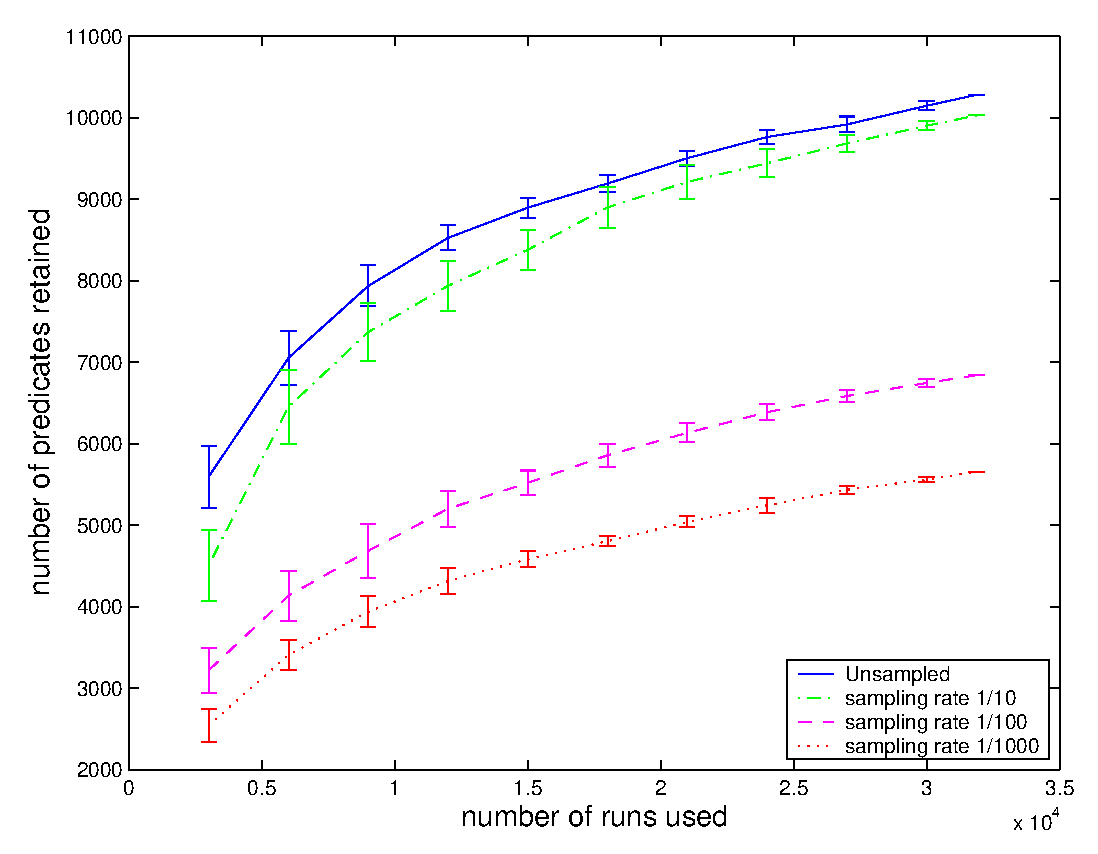
\includegraphics[width=\columnwidth]{predkept3a}\label{fig:predkept-a}}
  \hfill
  \subfigureautorefname[branches and returns only]{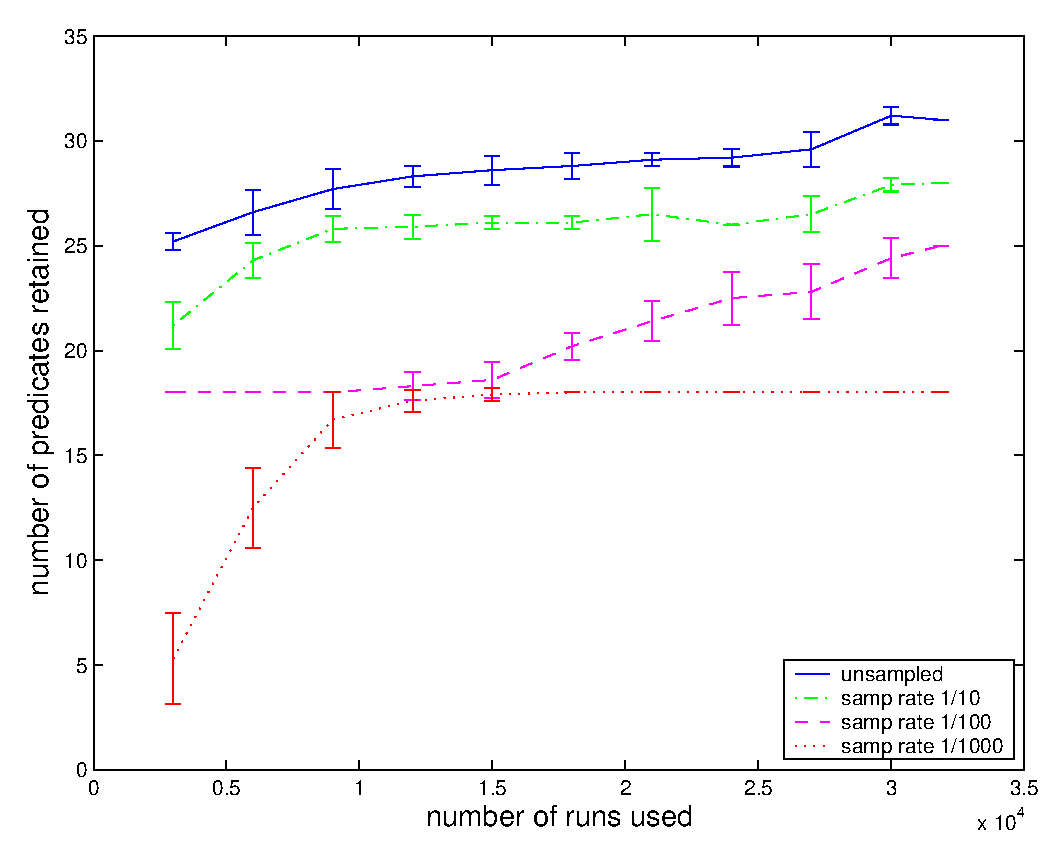
\includegraphics[width=\columnwidth]{predkept3b}\label{fig:predkept-b}}

  \caption{The effect of sampling and data size on the number of
  predicates selected.}\label{fig:predkept}
\end{figure*}

Two trends are apparent from \Autoref{fig:predkept}.  As one would expect,
the number of retained predicates decreases as the sampling rate decreases,
and increases as more trial runs are included.  If we had an unlimited number
of trial runs, the number of retained predicates at all sampling rates should
approach the result with no sampling.  

Note also that increasing 
the number of trial runs always seems to increase the number of retained 
scalar-pairs predicates, whereas the branch and returns predicates run into 
a plateau at lower sampling rates.  Though there may not be much significance 
in this discovery, we conjecture that it is due to the fact that scalar
pairs predicates are much more often observed than the other two kinds of
predicates.  Therefore determining the importance of scalar pairs predicates
takes much fewer sampled trial runs.

%% As is apparent from the graph, there is much larger variation in the
%% number of selected predicates when we use fewer trial runs.
%% %Using $3000$ trials, at the minimum we
%% %retain $7429$ predicates using unsampled data, $7654$ when sampling
%% %rate is $\nicefrac{1}{10}$, $7347$ at $\nicefrac{1}{100}$, and $6750$
%% %at $\nicefrac{1}{1000}$;
%% As we incorporate more examples of successful and failed \moss\ runs,
%% the variances decrease for all sampling rates, but the means behave
%% somewhat differently.  When the data is not sampled, the average
%% number of selected predicates stays around $8100$ for all data sizes.
%% Sampling adds noise to this procedure.  As we observed previously,
%% a moderate sampling rate tends to drive up the $\increase(\ldots)$ scores, and
%% thus enlarges our set of selected predicates (except when we are using
%% very few trial runs).

%% At the relatively high sampling rate of
%% \nicefrac{1}{10}, there are still enough samples taken at most
%% instrumentation sites, and there is a net increase in the number of
%% selected predicates.  Once the sampling rate shrinks to
%% \nicefrac{1}{100} and below, however, the effect of sparse
%% sampling sets in.  Fewer samples are taken overall on fewer predicates,
%% and as a result, fewer predicates have a nonzero $\increase(\ldots)$ score.
%% Incorporating more runs tends to alleviate the situation; at above
%% 10,000 runs, roughly the same number of predicates are retained for
%% the \nicefrac{1}{100} sampled data as the complete data.  The very
%% sparse sampling rate of \nicefrac{1}{1000}, on the other hand,
%% causes much more change in the final result.  A lot more predicates
%% are eliminated when using fewer trials, and a lot more predicates are
%% retained using more trials.

%% Most of the volatility in the results come from the scalar-pair
%% predicates.  \Autoref{fig:predkept-b} shows the same graph for
%% only the branch and return predicates.  Here, across all data sizes,
%% the number of selected predicates remains roughly constant at each
%% sampling rate.  The complete data is still able to select the fewest
%% number of predicates, with \nicefrac{1}{100} sampled data following
%% close behind.  The \nicefrac{1}{1000} sampled data still produces a
%% net increase in the number of selected predicates.

%% LocalWords:  downsampling lang downsampled predelim predkept

% -*- TeX-master: "master" -*-

\section{Related Work}
\label{sec-related-work}
Daikon \cite{ErnstCGN2001:TSE} detects invariants in a program by observing multiple program runs.  Invariants are predicates generated using operators like sum, max, etc.\ to combine program variables and collection (e.g., array) objects.  Daikon is intended for many uses beyond bug isolation, and so it monitors a much larger set of predicates than CBI.  This makes scalable complex predicate generation more difficult.  However, Dodoo et al.\ \cite{ErnstDRAFT} have successfully extended the work to generate implications from the simpler, measured predicates.  Dodoo et al.\ alternate clustering and invariant detection to find invariant implications over a set of program runs.  The initial clustering is performed using the $k$-means algorithm \cite{jain99data}, with program runs represented as normalized vectors of scalar variable values.  Since CBI represents run information as bit-vectors this technique can be applied essentially unchanged.

Daikon's implication generation extends its vocabulary of possible invariants.  CBI's focus is detection of bug predictors, which under sparse sampling conditions can rarely be identified as invariant.  Additionally, the existence of an implication is of questionable value in this project; the implication revealed in \autoref{sec-ccrypt} is an interesting and potentially useful side-effect of our analysis, but only because it involves identified bug predictors.  The approach described in this paper is better suited to the goals and analysis techniques of CBI\@.  There are no known attempts to use Daikon under sparse sampling conditions.

DIDUCE \cite{581377} detects invariant bits of program values during an initial training phase.  During the checking phase, DIDUCE reports each invariant violation as it occurs, then relaxes the invariant to accept the new value.  Unlike Daikon and CBI, DIDUCE tightly couples data collection and evaluation.  Because of this coupling, neither our nor Daikon's offline style of predicate generation is readily combined with DIDUCE's framework.

Haran et al.\ \cite{haran05TCEDS} analyze data from deployed software to classify executions as \emph{success} or \emph{failure}.  They use tree based classifiers and association rules to model ``failure signals.''  Tree based classifiers can encode both conjunctions and disjunctions whereas association rules cannot encode disjunctions when limited to a constant size.

SOBER \cite{1081753} is a statistical debugging tool similar to CBI\@.  Where CBI considers only whether a predicate was ever observed true during an execution, SOBER estimates the likelihood of it being true at any given evaluation.  SOBER data is a probability vector, with each value representing the estimated chance of a simple predicate being true when observed.  The similarity in collected data means that similar techniques for complex predicate generation are applicable.  The three-valued logic described in \autoref{sec-tvl} could be replaced with joint-probability when generating conjunctions; De Morgan's law can be applied to generate disjunctions.  Our usability metrics can be used on the resulting data.  There are no known experiments using SOBER under sparse sampling conditions.  Complex predicate generation removes a key advantage of SOBER: predicate scores result directly from the number of actual predicate evaluations.  Complex predicates generated by this technique are never truly evaluated, so their probability values would have little connection to actual program execution.  Whether this would affect their usefulness is unknown.

% LocalWords:  Dodoo Daikon's ccrypt DIDUCE DIDUCE's tvl

% -*- TeX-master: "master" -*-
%       *         *         *         *         *         *         *         *

\section{Conclusion}
\label{sec-conclusion}
We have demonstrated that complex predicates are useful predictors of bugs.  
Our experiments show qualitative and quantitative evidence that the statistical 
analysis used by CBI can be effectively applied to compound predicates, and that
the resulting analysis provides improved results.  We describe
two methods of eliminating predicate combinations from consideration, making
the task of computing complex predicates more feasible.  First is a numeric 
estimate on the upper bound of the score of a complex predicate.  The second is 
a metric that quantifies the usefulness of a complex predicate.  Even after these, 
the computational complexity is still high and requires further improvements.  
The metrics described in \autoref{sec-metrics} help select the most useful predicates
from those generated.  But the metrics are not perfect as finding a good candidate
for use in debugging requires sifting through a large number of less useful predicates
that also passed automated inspection.  Most such predicates are redundant predictors
for the same set of program failures, and so the bi-clustering algorithm of Zheng et al.\ 
\cite{Zheng:2006:SDSIMB} may solve this problem as it was designed with the goal 
of handling multiple predictors for the same bug.

% -*- TeX-master: "report" -*-

\section*{Acknowledgments}

We would like to thank Anne Mulhern for her insightful comments on an earlier draft of this paper.


\bibliographystyle{abbrv}
\bibliography{local}

\end{document}
